%\documentclass[10pt,a4paper]{article}
\documentclass[10pt,a4paper]{scrreprt}
\usepackage[utf8]{inputenc}
\usepackage{amsmath}
\usepackage{amsfonts}
\usepackage{amssymb}
\usepackage{graphicx}
\usepackage{subfigure}
\usepackage[left=2cm,right=2cm,top=2cm,bottom=2cm]{geometry}

\usepackage{bm}

\usepackage{pythonhighlight}

% integral d
\newcommand{\myd}{\;\mathrm{d}}
% overbar
\newcommand{\overbar}[1]{\mkern 1.5mu\overline{\mkern-1.5mu#1\mkern-1.5mu}\mkern 1.5mu}

\author{Yi Hu}
\title{Homogenization for Multi Field Modelling}
\subtitle{Part II: Implementation and Numerical Examples}

\begin{document}

\chapter{Numerical Examples}
In this part some numerical examples using this module is presented. First different kinds of inclusions are listed. Then 2d and 3d examples both in uni field and multi field modelling are given. At the end of this part the usage of the module is given in the IPython environment.

\section{Various Inclusions}
Inclusions in two dimensional or three dimensional cases can be added to the unit cell. User defined mesh and geometry can also be applied.

\begin{figure}[h]
  \centering
  \subfigure[2D Circle Inclusion]{
    \label{fig: inc 2d circ} %% label for first subfigure
    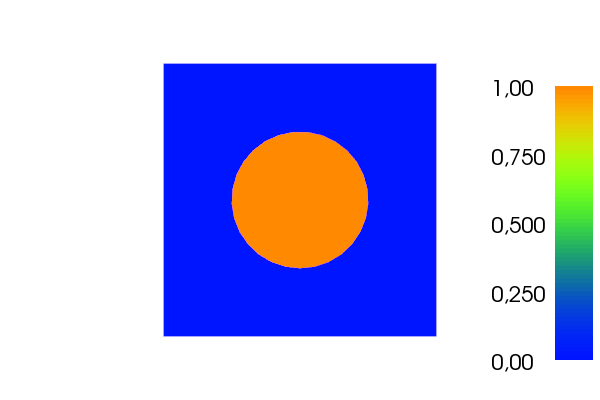
\includegraphics[width=0.45\linewidth]{../pics/dolfin_plot_0.png}}
  %\hspace{0in}
  \subfigure[3D Unit Cube with Inclusion at Corners]{
    \label{fig: inc 3d box} %% label for second subfigure
    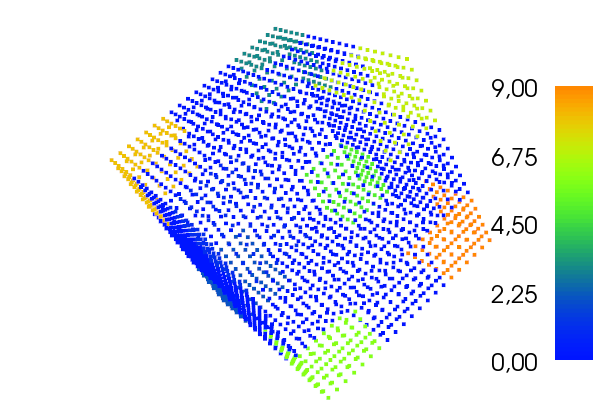
\includegraphics[width=0.45\linewidth]{../pics/dolfin_plot_2.png}}
  \caption{Various Inclusion Types}
  \label{fig: inc} %% label for entire figure
\end{figure} 

\section{2D Modelling}
\subsection{Uni Field Modelling}
A unit square is considered in two dimensional calculation. At first a uni field problem is introduced, specifically a Saint Venant-Kirchhoff material in mechanical field. The model is given in the previous chapter. Material parameters and geometry parameters are given in the following table. The inclusion is simply a center located circle with radius 0.25. \\

\begin{figure}[h]
  \centering
  \subfigure[Coarse Mesh]{
    \label{fig: inc 2d circ}
    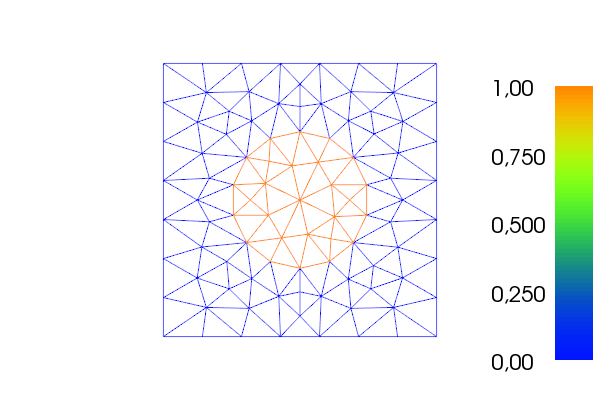
\includegraphics[width=0.45\linewidth]{../pics/dolfin_plot_16.png}}
  %\hspace{0in}
  \subfigure[Fine Mesh]{
    \label{fig: inc 3d box}
    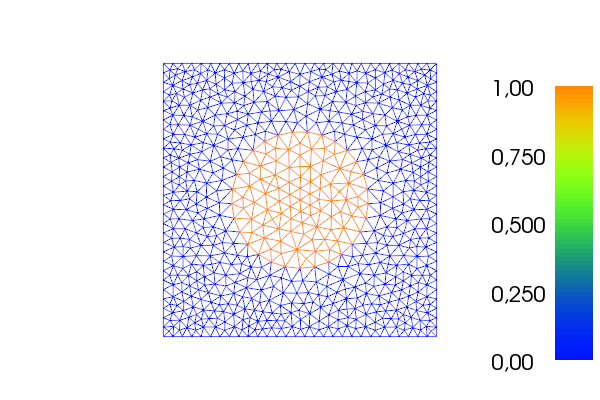
\includegraphics[width=0.45\linewidth]{../pics/dolfin_plot_15.png}}
  \caption{Geometry Layout and Mesh}
  \label{fig: inc}
\end{figure} 

\begin{center}
\captionof{table}{Material Parameters}
\begin{tabular}{l|c|c}
\hline
& Young's Modulus & Poisson Ratio \\
\hline
Matrix Material & 10.0 & 0.3 \\
Inclusion Material & 1000.0 & 0.3 \\
\hline
\end{tabular}
\end{center}
Boundary condition is periodic boundary condition and the fluctuation at corners is fixed to prevent rigid body movements. And the macro field is set as 
\[
\overbar{\mathbf{F}} = 
\begin{bmatrix}
0.9 & 0 \\
0 & 1 \\
\end{bmatrix},
\]
which is an uni axial compression test. Here the macro deformation is set not very large. Because of the non-linearity nature of the problem, the load cannot set to be too high. For large macro deformation input a quasi static loading process needs to be imposed. This will achieve more obvious loading. The fluctuation plot, strain plot and stress plot is demonstrated here.

\begin{figure}[h]
  \centering
  \subfigure[Coarse Mesh Contour on Element]{
    \label{fig: inc 2d circ}
    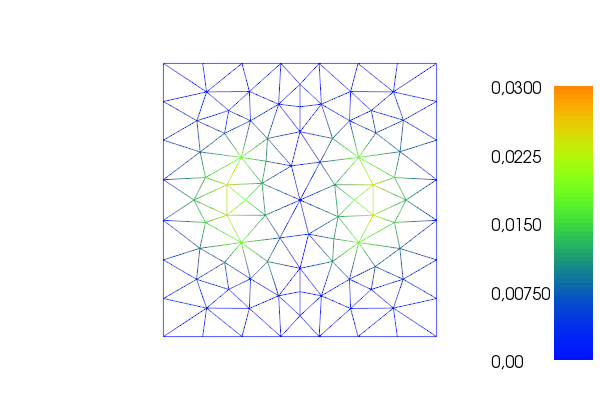
\includegraphics[width=0.45\linewidth]{../pics/dolfin_plot_5.png}}
  %\hspace{0in}
  \subfigure[Coarse Mesh Fluctuation Contour]{
    \label{fig: inc 3d box}
    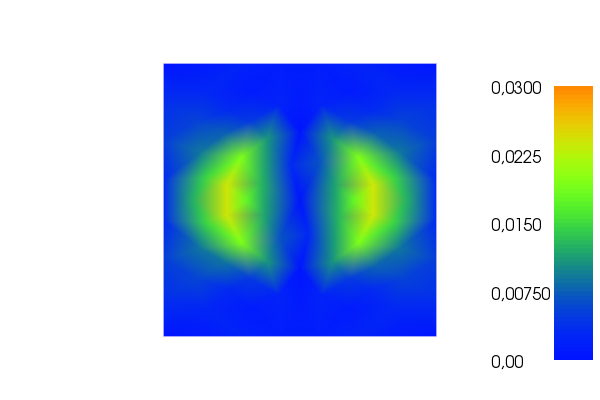
\includegraphics[width=0.45\linewidth]{../pics/dolfin_plot_3.png}}
  \label{fig: inc} 
  \subfigure[Fine Mesh Contour on Element]{
    \label{fig: inc 2d circ}
    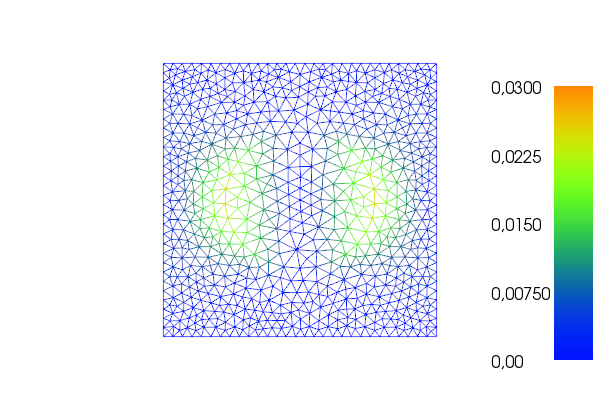
\includegraphics[width=0.45\linewidth]{../pics/dolfin_plot_4.png}}
  %\hspace{0in}
  \subfigure[Fine Mesh Fluctuation Contour]{
    \label{fig: inc 3d box}
    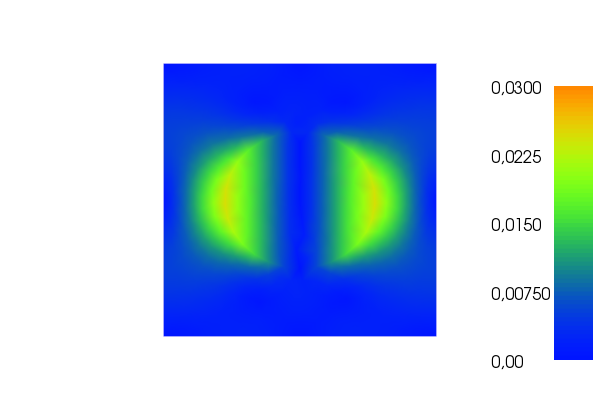
\includegraphics[width=0.45\linewidth]{../pics/dolfin_plot_6.png}}
  \caption{Uniaxial Compression Test: Fluctuation Result}
\end{figure} 

If shear macro field strain is defined, namely
\[
\overbar{\mathbf{F}} = 
\begin{bmatrix}
1. & 0.5 \\
0 & 1 \\
\end{bmatrix},
\]
the result will look like 

\begin{figure}[h]
  \centering
  \subfigure[Coarse Mesh Contour on Element]{
    \label{fig: inc 2d circ}
    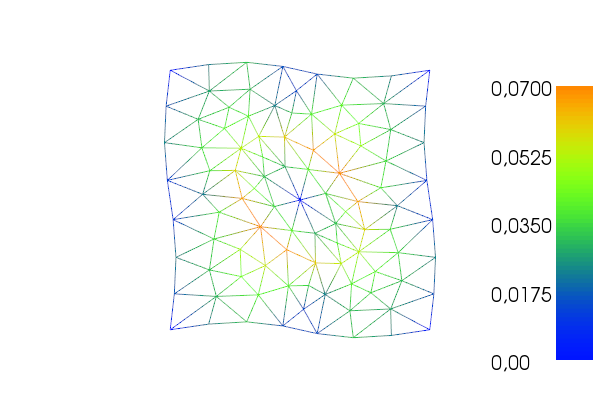
\includegraphics[width=0.45\linewidth]{../pics/dolfin_plot_9.png}}
  %\hspace{0in}
  \subfigure[Coarse Mesh Fluctuation Contour]{
    \label{fig: inc 3d box}
    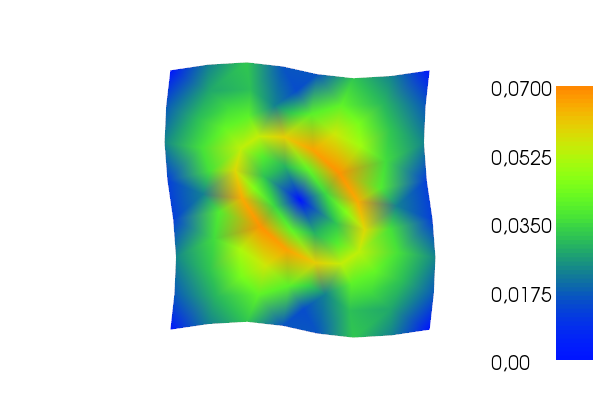
\includegraphics[width=0.45\linewidth]{../pics/dolfin_plot_8.png}}
  \label{fig: inc} 
  \subfigure[Fine Mesh Contour on Element]{
    \label{fig: inc 2d circ}
    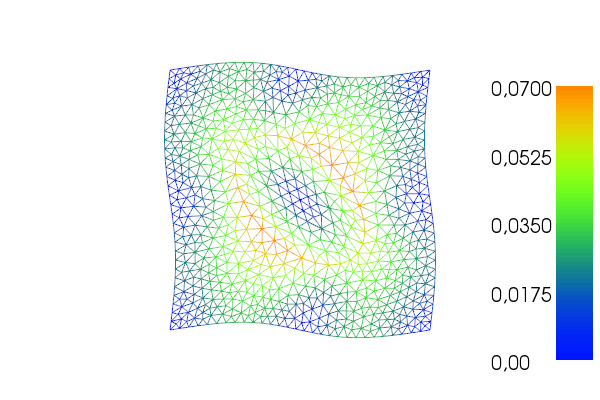
\includegraphics[width=0.45\linewidth]{../pics/dolfin_plot_11.png}}
  %\hspace{0in}
  \subfigure[Fine Mesh Fluctuation Contour]{
    \label{fig: inc 3d box}
    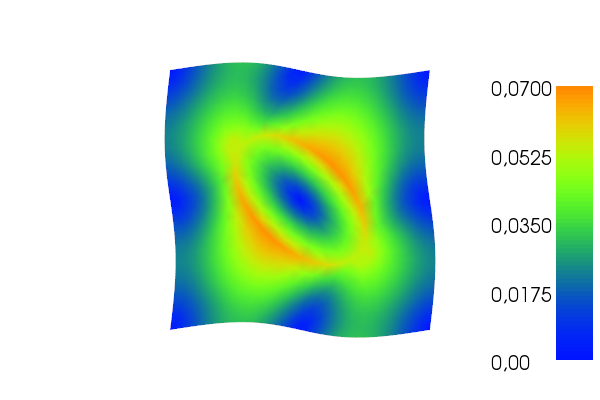
\includegraphics[width=0.45\linewidth]{../pics/dolfin_plot_10.png}}
  \caption{Simple Shear Test: Fluctuation Result}
\end{figure}

The calculated homogenized tangent moduli (from fine mesh) for uniaxial compression load case is 
\begin{equation}
\mathbb{C}_{\text{eff}} = 
\begin{bmatrix}
1.05215604 \times 10^{+01} &  6.81100019\times 10^{-04}  & 8.10922941\times 10^{-04} & 6.0931974\times 10^{+00} \\
6.81100019\times 10^{-04} &  3.03957695\times 10^{+00} &  4.12022593\times 10^{+00} & -2.43801203\times 10^{-04}\\
8.10922941\times 10^{-04} &  4.12022593\times 10^{+00} &  2.98311033\times 10^{+00} & -3.19622254\times 10^{-04}\\
6.09319740\times 10^{+00} & -2.43801203\times 10^{-04} & -3.19622254\times 10^{-04} &  1.74423266\times 10^{+01}\\
\end{bmatrix},
\end{equation}
while for simple shear load case is 
\begin{equation}
\mathbb{C}_{\text{eff}} = 
\begin{bmatrix}
22.27828078 & 11.45747779 &  4.84645322 &  7.52308193 \\
11.45747779 & 15.71048687 &  6.80879894 & 11.93754869 \\
4.84645322 &  6.80879894  & 7.35347903 &  4.53857874 \\
7.52308193 & 11.93754869 &  4.53857874 & 23.42982073 \\
\end{bmatrix},
\end{equation}

Comment: Stress and strain plot is not smooth!! And is throws the error that it cannot plot properly.


\subsection{Multi Field Modelling}
As for multi field modelling, the material considered is Neo Hookean type electroactive polymer material in both mechanical and electrical fields, 
\begin{equation}
\label{eq: nhk}
\psi\left( \mathbf{C}, \mathbf{E} \right) =  \frac{1}{2}\mu_{0} \left( \text{tr}[\mathbf{C}]-3 \right) + \dfrac{\lambda}{4} \left( J^{2}-1 \right) - \left( \dfrac{\lambda}{2} + \mu \right) \ln J - \frac{1}{2} \epsilon_{0} \left( 1+\dfrac{\chi}{J} \right) J \left[ \mathbf{C}^{-1}: (\mathbf{E} \otimes \mathbf{E}) \right]
\end{equation}
Macro field input is 
\[
\overbar{\mathbf{F}} = 
\begin{bmatrix}
0.9 & 0 \\
0 & 1 \\
\end{bmatrix},
\overbar{\mathbf{E}} = 
\begin{bmatrix}
0. \\
0.2
\end{bmatrix}
\]

Material input is in the following table,
\begin{center}
\captionof{table}{Material Parameters}
\begin{tabular}{l|c|c|c}
\hline
& Young's Modulus & Poisson Ratio & Electric Susceptibility\\
\hline
Matrix Material & $2\times 10^{5}$ & 0.4 & 7 \\
Inclusion Material & $2\times 10^{8}$ & 0.3 & 7000 \\
\hline
\end{tabular}
\end{center}

The fluctuation result is illustrated below (only the fine mesh is given). And the effective tangent moduli is
\begin{equation}
\mathbb{C}_{\text{eff}} = 
\begin{bmatrix}
[[  1.26964757e+06  -1.68087536e+00  -2.02332432e+00   1.05514398e+06
   -1.57805309e+00  -1.31326835e+04]
 [ -1.68087536e+00   3.23090783e+05   4.41338179e+03  -1.13998687e+00
   -1.70067902e+04   1.95527770e+00]
 [ -2.02332432e+00   4.41338179e+03   3.27056466e+05  -1.12653621e+00
   -1.88964336e+04   2.17253080e+00]
 [  1.05514398e+06  -1.13998687e+00  -1.12653621e+00   1.51218863e+06
    2.25985680e+00  -4.69241135e+04]
 [ -1.57805309e+00  -1.70067902e+04  -1.88964336e+04   2.25985680e+00
    1.16854722e+05   3.48372831e+00]
 [ -1.31326835e+04   1.95527770e+00   2.17253080e+00  -4.69241135e+04
    3.48372832e+00   9.72390167e+04]]
\end{bmatrix}.
\end{equation}

\begin{figure}[htbp]
  \centering
  \subfigure[Fluctuation of Displacement on Element Edges]{
    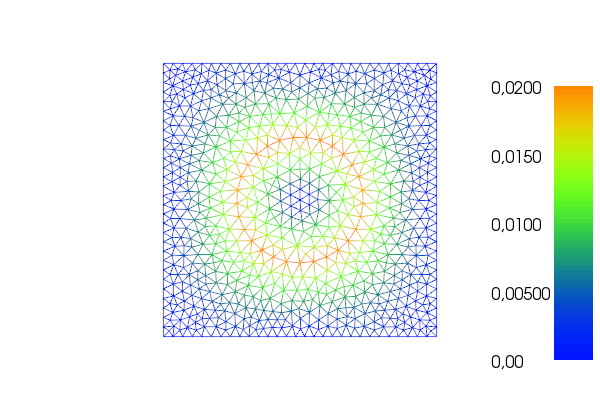
\includegraphics[width=0.45\linewidth]{../pics/multi_field_disp2.png}}    
  \subfigure[Fluctuation of Displacement]{
    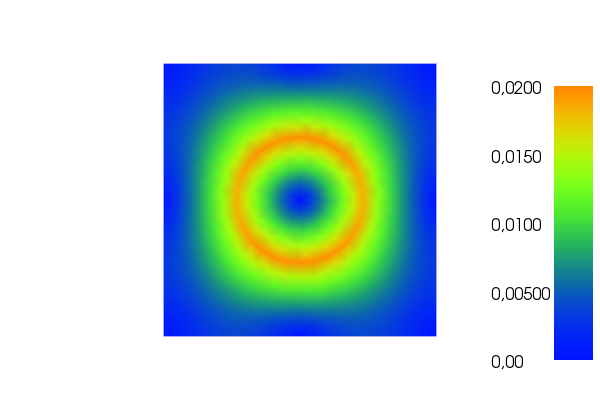
\includegraphics[width=0.45\linewidth]{../pics/multi_field_disp.png}}
  \subfigure[Fluctuation of Electrical Potential on Element Edges]{
    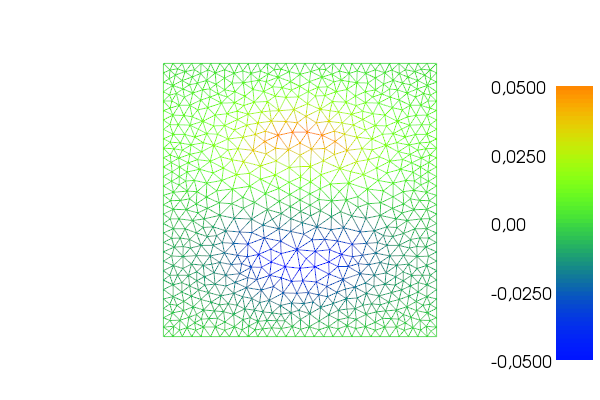
\includegraphics[width=0.45\linewidth]{../pics/multi_field_pot2.png}}
  \subfigure[Fluctuation of Electrical Potential]{
    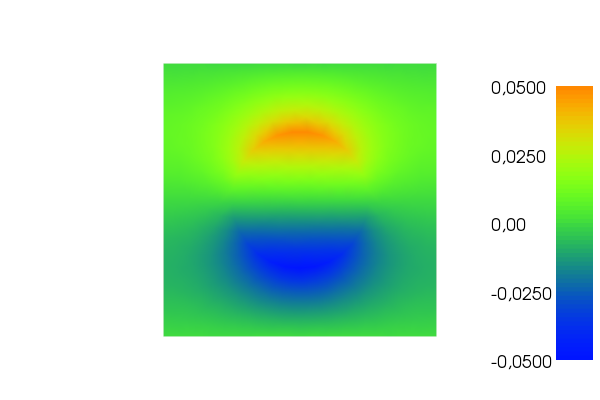
\includegraphics[width=0.45\linewidth]{../pics/multi_field_pot.png}}
  \subfigure[Electrical Field Intensity in Y Direction on Element Edges]{
    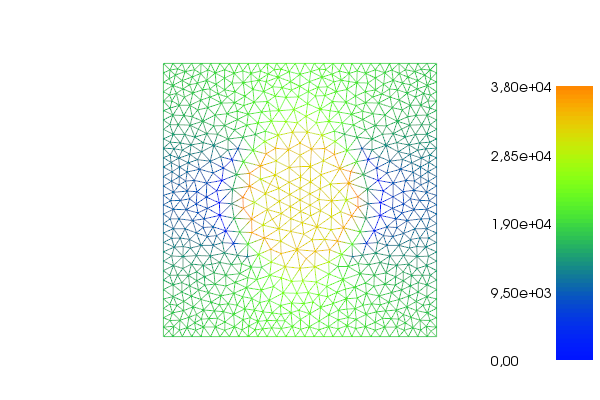
\includegraphics[width=0.45\linewidth]{../pics/multi_field_el2.png}}
  \subfigure[Electrical Field Intensity in Y Direction]{
    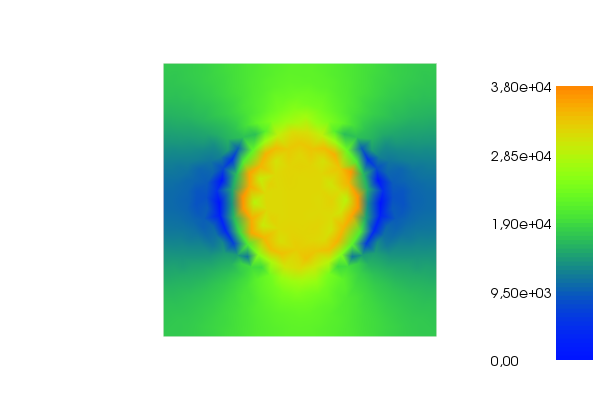
\includegraphics[width=0.45\linewidth]{../pics/multi_field_el.png}}
  \caption{Multi Field Modelling: Electroactive Polymer in Mechanical Field and Electrical Field}
\end{figure}

\newpage
\section{3D Modelling}
In 3D case we consider a unit cube, where a rectangular block is set as inclusion which cuts through the unit cell. Uni field and multi field problems are both accounted in this circumstance. Material parameters are set as the same with in 2D cases, while the macro field input for uni field and multi field are as follows.



[fig: 3d uni]

[fig: 3d multi]

\section{Simulation Template}
In this section a simulation template is provided. The presentation of this template introduces all the common interface of this module, which allows users to gain an overview of all the usages of this module. This code sample starts with importing all the files of unit cell module. Then geometry is defined within \texttt{cell\_geom.py} followed with material definition within \texttt{cell\_material.py}. Completing the setting of the problem calculation is initiated with defining an object of \texttt{MicroComputation} from \texttt{cell\_computation.py}. After inputting macro field and field variables which need to be solved, micro fluctuation can be calculated using the member method \texttt{comp\_fluctuation()} and the user defined solver parameters. It is seen that an instance of \texttt{MicroComputation} can be called every time step and reused among several different cells if the setting of geometry and materials does not change. The only thing to notice is that a new FEniCS \texttt{Function} object should be provided in the interim. This template can be used in IPython interactively or embedded in other computation which requires a unit cell investigation.

\begin{python}
from dolfin import *

import numpy as np

# Module files
import cell_geom as geom
import cell_material as mat
import cell_computation as comp

# Set linear algebra backend, supported are Eigen and PETSc
parameters['linear_algebra_backend'] = 'Eigen'

# Geometry definition
mesh = Mesh(r'./m_fine.xml')
cell = geom.UnitCell(mesh)
inc = geom.InclusionCircle(2, (0.5, 0.5), 0.25)
inc_di = {'circle_inc': inc}
cell.set_append_inclusion(inc_di)

# Material definition
E_m, nu_m, E_i, nu_i = 10.0, 0.3, 1000.0, 0.3
mat_m = mat.st_venant_kirchhoff(E_m, nu_m)
mat_i = mat.st_venant_kirchhoff(E_i, nu_i)
mat_li = [mat_m, mat_i]

# Fields definition
VFS = VectorFunctionSpace(cell.mesh, "CG", 1, 
                          constrained_domain=geom.PeriodicBoundary_no_corner(2))

def deform_grad_with_macro(F_bar, w_component):
    return F_bar + grad(w_component)

w = Function(VFS)
strain_space = TensorFunctionSpace(mesh, 'DG', 0)

# Micro Computation instantiation
compute = comp.MicroComputation(cell, mat_li, 
                                [deform_grad_with_macro],
                                [strain_space])

# Input macro field and field variable
F_bar = [0.9, 0., 0., 1.]
compute.input([F_bar], [w])

# Set linear solver and parameters and solve the problem
comp.set_solver_parameters('non_lin_newton', lin_method='direct',
                      linear_solver='cholesky')
compute.comp_fluctuation(print_progress=True, print_solver_info=False)

compute.view_fluctuation()

# Load step
delta = 0.01

# Calculate with different load steps
for i in range(10):
    F_bar[0] -= delta
    print F_bar
    compute.input([F_bar], [w])
    compute.comp_fluctuation(print_progress=True, print_solver_info=False)
\end{python}

\section{Convergence Comparison with Finite Difference Calculation}
The convergence of the homogenized effective tangent moduli is investigated with Finite Difference calculation. Here Finite Difference calculation stands for the difference of the averaged extended stress with respect to small change of the macro extended strain input. This method leads to the following expression, 
\begin{equation}
\mathbb{C}_{\text{eff}} = \dfrac{\partial \mathbf{P}_{\text{avg}} \left( \overbar{\mathbf{F}}, \widetilde{\mathbf{F}} \right)}{\partial \overbar{\mathbf{F}}} \ \Rightarrow \ \mathbb{C}_{\text{eff}} = \dfrac{\Delta \mathbf{P}_{\text{avg}}}{\Delta \overbar{\mathbf{F}}}.
\end{equation}
The fraction of vectors or matrices is arranged in the same manner with the effective tangent moduli. In the calculation varying only a component of $\overbar{\mathbf{F}}$ is realized and the change of $\mathbf{P}_{\text{avg}}$ is calculated. The division ends with corresponding terms in $\mathbb{C}_{\text{eff}}$.

The result shows that in uni field and multi fields the implementation of the previous derivation gives a good approximate to the Finite Difference calculation of effective tangent moduli. The script for multiple fields modelling is given here.

\begin{python}
import sys
sys.path.append(r'../')

from dolfin import *
import numpy as np

import cell_computation as com
import cell_geom as ce
import cell_material as ma
from copy import deepcopy

import logging
logging.getLogger('FFC').setLevel(logging.WARNING)

# Geometry definition
mesh = Mesh(r"../m.xml")
cell = ce.UnitCell(mesh)
inc = ce.InclusionCircle(2, (0.5, 0.5), 0.25)
inc_di = {'circle_inc': inc}
cell.set_append_inclusion(inc_di)

# Electroactive polymer material model
E_m, nu_m, Kappa_m = 2e5, 0.4, 7.
n = 1000  
E_i, nu_i, Kappa_i = 1000 * E_m, 0.3, n * Kappa_m

mat_m = ma.neo_hook_eap(E_m, nu_m, Kappa_m)
mat_i = ma.neo_hook_eap(E_i, nu_i, Kappa_i)
mat_li = [mat_m, mat_i]

# Field variables
VFS = VectorFunctionSpace(cell.mesh, "CG", 1,
                          constrained_domain=ce.PeriodicBoundary_no_corner(2))
FS = FunctionSpace(cell.mesh, "CG", 1,
                   constrained_domain=ce.PeriodicBoundary_no_corner(2))
w = Function(VFS)
el_pot_phi = Function(FS)
strain_space_w = TensorFunctionSpace(mesh, 'DG', 0)
strain_space_E = VectorFunctionSpace(mesh, 'DG', 0)

def deform_grad_with_macro(F_bar, w_component):
    return F_bar + grad(w_component)
def e_field_with_macro(E_bar, phi):
    return E_bar - grad(phi)

# Computation initiation
comp = com.MicroComputation(cell, mat_li,
                        [deform_grad_with_macro, e_field_with_macro],
                        [strain_space_w, strain_space_E])

# Wrap for calculating averaged stress
def avg_mer_stress(F_bar, E_bar):
    comp.input([F_bar, E_bar], [w, el_pot_phi])
    comp.comp_fluctuation()
    return comp.avg_merge_stress()
    
# Calculate the corresponding components and stack them into a matrix
def conv_check_component(label, compo, delta):
    C_eff_component_FD = np.zeros(shape=(len(delta),6), dtype=float)
    if label is 'F':
        for i, d in enumerate(delta):
            F_minus = deepcopy(F_bar)
            F_minus[compo] = F_bar[compo] - d/2
            F_plus = deepcopy(F_bar)
            F_plus[compo] = F_bar[compo] + d/2

            P_minus = avg_mer_stress(F_minus, E_bar)
            P_plus  = avg_mer_stress(F_plus, E_bar)
            
            C_eff_component_FD[i,:] = (P_plus - P_minus)/d
    elif label is 'E':
        for i, d in enumerate(delta):
            E_minus = deepcopy(E_bar)
            E_minus[compo] = E_bar[compo] - d/2
            E_plus = deepcopy(E_bar)
            E_plus[compo] = E_bar[compo] + d/2

            P_minus = avg_mer_stress(F_bar, E_minus)
            P_plus  = avg_mer_stress(F_bar, E_plus)
            
            C_eff_component_FD[i,:] = (P_plus - P_minus)/d
    else:
        raise Exception('no such field label')
    
    return C_eff_component_FD 

# Macro field input
F_bar = [1.1, 0., 0.1, 1.]
E_bar = [0., 0.2]

# Finite difference step
delta = [0.01, 0.01/2, 0.01/4, 0.01/8]

# Finite difference calculation (the fourth component of C_eff)
C_eff_component_FD = conv_check_component('F', 3, delta)

# Homogenization calculation 
comp = com.MicroComputation(cell, mat_li,
                        [deform_grad_with_macro, e_field_with_macro],
                        [strain_space_w, strain_space_E])
comp.input([F_bar, E_bar], [w, el_pot_phi])
comp.comp_fluctuation()
C_eff = comp.effective_moduli_2()

# Observe the difference
component = C_eff[:,3]
tmp = np.outer(np.ones((len(delta),1)),np.transpose(component))
error = np.linalg.norm(tmp - C_eff_component_FD, axis=1)/np.linalg.norm(component)
\end{python}

The output of the error (or calculation difference between two methods) is in the following code block.
\begin{python}
In [61]: error

Out[61]:
array([  9.12302965e-06,   2.28075104e-06,   5.70186024e-07,
         1.42533577e-07])
\end{python}

The result shows that the homogenized solution of effective tangent moduli is in good agreement with the one calculated from Finite Difference method in both uni field case and multi field case. 

\end{document}

